\documentclass[10pt]{article}
\usepackage[margin=0.78in]{geometry}
\usepackage{amsmath,amssymb,amsthm,mathtools,bm}
\usepackage{booktabs,tabularx,array,microtype,graphicx}
\usepackage{enumitem,float,placeins}
\usepackage[numbers,sort&compress]{natbib}
\usepackage{xcolor}
\usepackage[colorlinks=true,allcolors=blue!55!black]{hyperref}
\usepackage[capitalize,noabbrev]{cleveref}

\newtheorem{theorem}{Theorem}
\newtheorem{proposition}{Proposition}
\newtheorem{corollary}{Corollary}
\newtheorem{assumption}{Assumption}
\newtheorem{definition}{Definition}
\newcommand{\R}{\mathbb R}
\newcommand{\E}{\mathbb E}
\newcommand{\Hh}{\mathcal H}
\newcommand{\U}{\mathcal U}
\newcommand{\D}{\mathcal D}
\newcommand{\G}{\mathcal G}
\newcommand{\ip}[2]{\left\langle #1,#2\right\rangle_n}
\newcommand{\normn}[1]{\left\lVert #1\right\rVert_{2,n}}
\newcommand{\norminf}[1]{\left\lVert #1\right\rVert_{\infty}}
\newcommand{\Rcal}{\mathcal R}
\newcommand{\supp}{\operatorname{supp}}
\setlist{nosep,leftmargin=*}
\renewcommand{\arraystretch}{1.12}

\title{\vspace{-1.4em}\textbf{From Predictive Uncertainty to
Decision-Effective Dynamics Ambiguity Sets}\\
\large Perturbation-Calibrated Function-Space Uncertainty for Robust PDE Control}
\author{Yaowen Kang\\
\small Department of Mathematics, Imperial College London}
\date{Preprint draft, \today}

\begin{document}
\raggedbottom
\maketitle

\begin{abstract}
Neural PDE surrogates are usually assessed by prediction error, whereas a
controller is affected by the component of model error that changes its
finite-horizon objective. This paper studies the interface between these two
objects: how can predictive uncertainty be converted into a dynamics
ambiguity set that is effective for control decisions? We train a residual
Fourier neural operator (FNO) and a replica on Gaussian-perturbed labels. Their
smoothed disagreement supplies a spatial scale, while a disjoint deployment
audit split supplies finite-sample calibration. The resulting normalized
$L^2$ ellipsoid and simultaneous coordinate box are field-valued dynamics
sets, not scalar error bars. Robust model predictive control (MPC) queries
their geometry either through exact support functions in the finite-horizon
adjoint direction or through projected-gradient adversarial rollouts. We prove
split-conformal marginal coverage on a fixed discretization, derive exact
ellipsoidal and box support functions and a second-order linearization
remainder, and establish multi-step rollout and discounted policy-transfer
bounds under a separate uniform one-step error assumption. The conformal and
uniform-error results are explicitly not merged. On controlled viscous
Burgers dynamics under parameter, boundary, initial-condition, and latent
actuator shifts, deployment calibration restores field coverage and changes
closed-loop tail cost in a geometry-dependent manner; the simultaneous-box
adjoint controller lowers empirical $p90$ cost by $10.84\%$ relative to
nominal MPC in 24 matched cases. An official two-dimensional Navier--Stokes
benchmark exposes the high-dimensional cost of simultaneous bands and weak
error localization. These results support an uncertainty-to-decision
mechanism, not a general safety certificate.
\end{abstract}

\section{Introduction}

Learned operators can replace repeated numerical solves inside planning and
control loops. Fourier neural operators (FNOs), DeepONets, and related neural
operators learn maps between discretized functions and have demonstrated fast
surrogate prediction for Burgers, Darcy, and Navier--Stokes systems
\cite{li2021fno} and \cite{lu2021deeponet}; broader operator-learning
foundations are developed in \cite{kovachki2023neuraloperator} and
\cite{boulle2024guide}.
Their speed addresses only one part of model-based control. Once a controller
optimizes actions through a learned propagator, it can amplify a small but
decision-aligned model error even when the average field error is low.

Predictive uncertainty quantification (UQ) does not by itself resolve this
problem. In a spatial field, a large residual in a dynamically inactive region
may barely change the cost, while a smaller residual near an actuator or a
high-value gradient can reverse the preferred action. Conformal prediction
(CP) can give distribution-free finite-sample coverage for a chosen score
under exchangeability \cite{angelopoulos2023gentle}; see also the foundational
treatment in \cite{vovk2005algorithmic}. However,
coverage specifies an event, not the action that should be taken. Conversely,
robust MPC requires an uncertainty geometry and repeatedly queries its support
along objective-sensitive directions. The scientific gap is therefore not
``how to attach error bars to an FNO'', but how to turn a calibrated
field-valued prediction set into a control object without overstating what the
coverage theorem guarantees.

We ask:
\begin{quote}
\emph{How can predictive uncertainty be converted into a dynamics ambiguity
set that is effective for control decisions?}
\end{quote}
Our answer is a three-stage construction: learn a local scale from sensitivity
to label perturbations; calibrate that scale on a disjoint deployment audit;
and query the resulting function-space set through the robust MPC objective.
The FNO is a replaceable world model rather than the architectural
contribution.

\subsection{Related work}

\paragraph{Operator learning and uncertainty.}
FNOs parameterize global integral kernels in Fourier space
\cite{li2021fno}, while the broader neural-operator framework formalizes
discretization-invariant maps between function spaces
\cite{kovachki2023neuraloperator}. DeepONet provides a complementary
branch--trunk construction \cite{lu2021deeponet}. Recent UQ work includes
deep ensembles under PDE shift \cite{mouli2024uq}, probabilistic neural
operators \cite{bulte2025probabilistic}, approximate Bayesian neural
operators \cite{magnani2025bayesian}, and linearized function-valued Gaussian
processes \cite{magnani2025luno}. These methods estimate structured
uncertainty, but Bayesian or ensemble dispersion is not automatically a
finite-sample coverage statement.

Conformal operator-learning methods address validity in different senses.
Risk-controlling quantile neural operators calibrate functional coverage
\cite{ma2024calibrated}; Conformalized-DeepONet wraps a DeepONet with
distribution-free bands \cite{moya2025conformalized}; and split CP has been
formulated directly in function space \cite{millard2025functionspace}. Most
closely, Wang et al. train clean-label and perturbed-label FNOs and calibrate a
max-type score for simultaneous Navier--Stokes fields in a data-scarce regime
\cite{wang2026perturbation}. We adopt the perturbation scale as a sample-efficient
starting point, then ask the downstream question left open by field coverage:
which calibrated geometry is useful for control?

\paragraph{Conformal prediction for robust decisions and control.}
Conformal uncertainty sets have been connected to robust optimization
\cite{johnstone2021conformal}. In control, Chee et al. combine receding-horizon
weighted CP, dynamic constraint tightening, and a predictive reference
generator \cite{chee2024conformal}; adaptive CP has also been used in motion
planning \cite{dixit2023adaptive}. SODA-MPC uses conformalized ensembles and
runtime OOD adaptation \cite{contreras2025soda}, while conformalized
system-level synthesis constructs OOD reachable tubes
\cite{srinivasan2026ood}. Those works target finite-dimensional state tubes,
constraints, or online drift. Our setting instead starts with a discretized
PDE field, compares multiple function-space geometries at a matched audit
budget, and uses the finite-horizon objective itself to query the set. We do
not inherit their sequential, feasibility, or safety guarantees.

\paragraph{Decision-aware model error.}
Value-aware model learning replaces uniform prediction quality with error
measured through downstream value \cite{farahmand2017value}; calibrated
model-based reinforcement learning likewise shows that uncertainty quality can
affect planning \cite{malik2019calibrated}. Simulation lemmas and Lipschitz
analyses propagate one-step model error to long-horizon value error
\cite{asadi2018lipschitz}. Distributionally robust model-based reinforcement
learning optimizes against dynamics ambiguity in large state spaces
\cite{ramesh2024drmbrl}. Our contribution is an explicit bridge among these
themes: conformal calibration constructs the field set, its support function
connects geometry to value sensitivity, and independent closed-loop tests
decide whether the construction is useful.

\begin{table}[t]
\centering
\scriptsize
\caption{Positioning relative to the closest lines of work. ``Field'' means a
joint object over a discretized PDE output; guarantee scopes are not directly
comparable.}
\label{tab:related}
\begin{tabularx}{\linewidth}{@{}p{0.17\linewidth}p{0.19\linewidth}p{0.23\linewidth}X@{}}
\toprule
Work & Uncertainty object & Decision interface & Main guarantee scope\\
\midrule
Ma et al. \cite{ma2024calibrated} & Functional quantile region & None & Risk-controlled functional coverage\\
Wang et al. \cite{wang2026perturbation} & Perturbation-scaled field box & None & Simultaneous discretized-field coverage\\
Chee et al. \cite{chee2024conformal} & Weighted-CP state intervals & Constraint tightening and reference generation & Time-varying model accuracy and robust constraints\\
Srinivasan et al. \cite{srinivasan2026ood} & Covariance-shaped OOD tube & System-level robust MPC & Weighted-CP OOD coverage and tube robustness\\
This work & Audit-calibrated $L^2$ ball, ellipsoid, and field box & Adjoint support or nonlinear adversarial MPC & One-step/behavior-rollout CP; separate deterministic value bound\\
\bottomrule
\end{tabularx}
\end{table}

\subsection{Contributions}

The paper makes four scoped contributions.
\begin{enumerate}[label=(\roman*)]
\item It defines a reproducible data pipeline from proper training through a
disjoint deployment audit to function-space dynamics sets. A clean-label FNO
and a perturbed-label replica use the full proper-training input set; no
calibration label trains either predictor.
\item It converts the sets into decision objects. We derive exact support
functions for normalized $L^2$ ellipsoids and coordinate boxes, use them in a
finite-horizon adjoint robust counterpart, and compare that approximation with
nonlinear projected-gradient adversarial rollouts.
\item It separates three kinds of theory: finite-sample marginal conformal
coverage, deterministic multi-step/value propagation under a uniform error
assumption, and a conditional curvature remainder for the first-order robust
objective. No one of these statements is used as a substitute for another.
\item It evaluates coverage, tightness, and control independently. Controlled
Burgers supplies closed-loop evidence under compound shift; the official
Navier--Stokes data supply a high-dimensional field-UQ stress test but no
control claim. Negative results are retained.
\end{enumerate}

\begin{figure}[H]
\centering
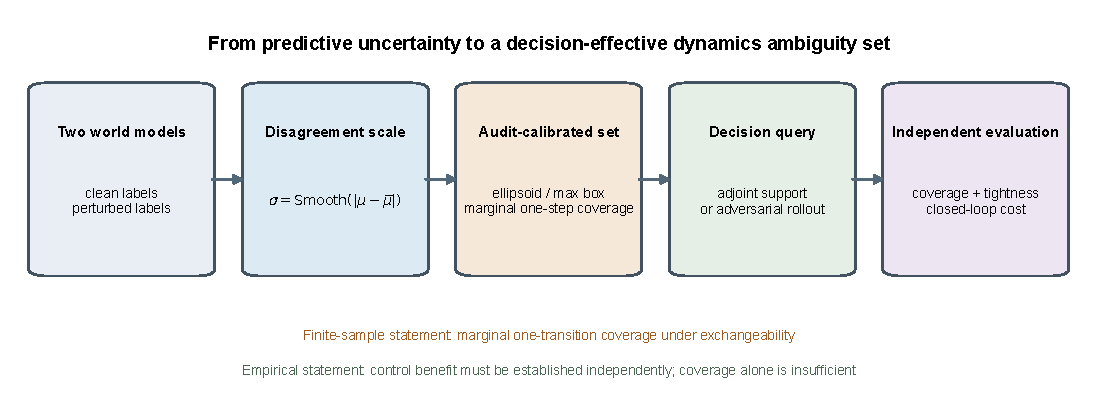
\includegraphics[width=\linewidth]{../../figures/method_01_chain_schematic.pdf}
\caption{Schematic of the proposed uncertainty-to-decision pipeline. Proper
training, deployment calibration, and independent evaluation use disjoint
data roles. The ambiguity set enters robust MPC through its support function
or a nonlinear adversarial rollout. The lower ledger prevents three statements
from being conflated: split-conformal field coverage, deterministic
uniform-error propagation, and empirical closed-loop benefit.}
\label{fig:schematic}
\end{figure}

\section{Preliminaries and problem setting}

\subsection{Controlled function-valued dynamics and discretization}

Let $u_t\in\Hh$ be a field on a spatial domain $\Omega$, let
$a_t\in\mathcal A\subset\R^p$ be a control, and let $\xi$ collect physical
parameters, boundary conditions, forcing, and unobserved actuator properties.
The deployment transition is
\begin{equation}
u_{t+1}=\G_\star(u_t,a_t;\xi).
\label{eq:continuous-dynamics}
\end{equation}
For computation, a projection $P_n:\Hh\to\R^n$ produces
$x_t=P_nu_t$. We write
\begin{equation}
x_{t+1}=G_{\star,n}(x_t,a_t;\xi),
\qquad
\ip{v}{w}=\frac{1}{n}\sum_{j=1}^{n}v_jw_j,
\qquad
\normn{v}^2=\ip{v}{v}.
\label{eq:discrete-dynamics}
\end{equation}
Nonuniform quadrature weights can replace $1/n$ without changing the
construction. Throughout, ``function-space set'' means a joint set for the
entire discretized field. Coverage on one fixed grid is not, by itself, a
continuum or grid-transfer guarantee.

The finite-horizon control cost is
\begin{equation}
J_H(x_0,a_{0:H-1})
=\sum_{t=1}^{H}\ell(x_t)+\sum_{t=0}^{H-1}r(a_t),
\label{eq:finite-cost}
\end{equation}
where low cost is preferred. A learned one-step propagator
$\widehat G_\theta$ is rolled out inside MPC and can therefore be queried at
states and actions induced by the optimizer rather than by the data-collection
policy.

\subsection{Data roles and deployment shift}

We distinguish four data roles:
\begin{align*}
\D_{\rm tr}&=\{(x_i,a_i,y_i)\}_{i=1}^{N_{\rm tr}},
&\D_{\rm val}&=\{(x_i,a_i,y_i)\}_{i=1}^{N_{\rm val}},\\
\D_{\rm cal}&=\{(x_i,a_i,y_i)\}_{i=1}^{m},
&\D_{\rm te}&=\{(x_i,a_i,y_i)\}_{i=1}^{N_{\rm te}}.
\end{align*}
Proper training and validation come from a source regime. The deployment audit
$\D_{\rm cal}$ is a small labeled sample from the target regime and is used
only to compute conformal order statistics. The test set remains untouched
until final evaluation. The clean and perturbed models, smoothing kernel, and
floor rule are measurable with respect to proper-training randomness and are
fixed before $\D_{\rm cal}$ is scored.

This is an \emph{audit-calibrated} setting: validity requires that calibration
and target examples are exchangeable after conditioning on the trained models.
If the deployment distribution changes again after the audit, ordinary split
CP does not protect against that new shift. Weighted or adaptive CP
\cite{barber2023beyond}, or covariate-shift calibration
\cite{tibshirani2019covariate}, is a possible extension, not a
guarantee claimed here.

\subsection{Split conformal prediction}

Let $Z_i=(X_i,A_i,Y_i)$ and let $S(Z_i)$ be a fixed scalar
nonconformity score. With calibration scores
$S_{(1)}\le\cdots\le S_{(m)}$, target miscoverage $\alpha\in(0,1)$,
and
\begin{equation}
k=\left\lceil (m+1)(1-\alpha)\right\rceil,
\qquad q_{1-\alpha}=S_{(k)},
\label{eq:cp-quantile}
\end{equation}
the standard convention sets $q_{1-\alpha}=+\infty$ if $k>m$. Equivalently,
the empirical distribution is augmented by an atom at $+\infty$. For a new
input $(x,a)$, the prediction set is
\begin{equation}
C(x,a)=\{y:S(x,a,y)\le q_{1-\alpha}\}.
\label{eq:cp-set}
\end{equation}
Under exchangeability, the rank of the new score among the $m+1$ scores yields
marginal coverage at least $1-\alpha$. The word \emph{marginal} matters: it is
not conditional coverage at every state--action pair and it is not automatic
simultaneous coverage over a counterfactual MPC rollout.

\subsection{Problem statement and decision effectiveness}

We seek a map from predictive scale to a dynamics set
$\U_\theta(x,a)\subset\R^n$, followed by a robust planning rule. A useful
construction must answer two different questions:
\begin{enumerate}[label=(P\arabic*)]
\item \textbf{Predictive validity and efficiency:} does the set attain its
predeclared coverage event on independent deployment data without unnecessary
width?
\item \textbf{Decision effectiveness:} at a matched world model and audit
budget, does using the set reduce paired mean cost, upper-tail cost, or
constraint violation relative to nominal planning and isotropic-set baselines?
\end{enumerate}

\begin{definition}[Decision-effective ambiguity set]
For a predeclared deployment distribution, controller, and downstream metric,
an ambiguity-set construction is decision-effective if its robust controller
improves that metric on independent matched closed-loop cases without violating
the accompanying mean-cost or feasibility criterion. Coverage is supporting
evidence, not the definition.
\end{definition}

\section{Methodology}

\subsection{Residual FNO world model}

The base one-step world model is a residual FNO,
\begin{equation}
\widehat G_\theta(x,a,\xi_{\rm obs})
=x+\delta_\theta(x,a,\xi_{\rm obs}).
\label{eq:residual-fno}
\end{equation}
For Burgers, the five input channels are the current field, the action
multiplied by a fixed actuator profile, viscosity, a linear extension of the
two boundary values, and the spatial coordinate. Each block applies a spectral
convolution and a pointwise linear map inside a ResNet-style skip connection.
The final boundary coordinates are projected exactly to the supplied Dirichlet
values. The full run uses width 32, 14 Fourier modes, four residual blocks, and
240,454 trainable parameters across the clean and perturbed operators.

FNO is chosen because it is a standard field propagator
\cite{li2021fno}; the broader framework is reviewed in
\cite{kovachki2023neuraloperator}. Nothing in the calibration or
robust-control construction requires Fourier layers. Replacing it by another
differentiable operator changes the mean and scale quality, not the logic of
the method.

\subsection{Perturbation-based uncertainty scale}

Following the stability principle used for data-scarce operator UQ
\cite{wang2026perturbation}, we train a second operator with the same
architecture and the same proper-training inputs but perturbed labels:
\begin{equation}
\widetilde y_i=y_i+\eta_i,
\qquad
\eta_i\stackrel{\rm iid}{\sim}\mathcal N(0,c^2s_y^2I_n).
\label{eq:label-perturbation}
\end{equation}
Let $\widetilde G_{\widetilde\theta}$ be its prediction. The raw disagreement,
smoothed disagreement, and stabilized scale are
\begin{align}
d(x,a)&=\left|\widehat G_\theta(x,a)-
\widetilde G_{\widetilde\theta}(x,a)\right|,\label{eq:raw-disagreement}\\
\bar d(x,a)&=K\ast d(x,a),\label{eq:smooth-disagreement}\\
\sigma(x,a)&=\bar d(x,a)\vee\tau_0.
\label{eq:scale}
\end{align}
The convolution is an odd moving-average window (five coordinates for
Burgers; $15\times15$ for Navier--Stokes). On Burgers, $\tau_0$ is $10\%$ of
the median interior disagreement on $\D_{\rm tr}$, lower bounded by $10^{-6}$.
Smoothing prevents isolated near-zero denominators from dominating a max-type
score; the floor is fixed before calibration. The raw scale has no coverage
interpretation. Split conformal calibration supplies validity.

\subsection{Perturbation-based nonconformity scores and calibration}

For residual $r=y-\widehat G_\theta(x,a)$, we compare three geometries.
\begin{align}
S_{\rm L2}(x,a,y)
&=\frac{\normn{r}}{\normn{\sigma(x,a)}},
\label{eq:l2-score}\\
S_{2}(x,a,y)
&=\normn{r\oslash\sigma(x,a)},
\label{eq:ell-score}\\
S_{\infty}(x,a,y)
&=\norminf{r\oslash\sigma(x,a)}.
\label{eq:max-score}
\end{align}
Here $\oslash$ denotes coordinate-wise division. Applying
\cref{eq:cp-quantile} separately gives $q_{\rm L2}$, $q_2$, and $q_\infty$.
The corresponding one-step dynamics sets are
\begin{align}
\U_{\rm L2}(x,a)
&=\left\{\widehat G_\theta(x,a)+\Delta:
\normn{\Delta}\le q_{\rm L2}\normn{\sigma(x,a)}\right\},
\label{eq:l2-set}\\
\U_2(x,a)
&=\left\{\widehat G_\theta(x,a)+\Delta:
\normn{\Delta\oslash\sigma(x,a)}\le q_2\right\},
\label{eq:ellipsoid-set}\\
\U_\infty(x,a)
&=\left\{\widehat G_\theta(x,a)+\Delta:
|\Delta_j|\le q_\infty\sigma_j(x,a),\ j=1,\ldots,n\right\}.
\label{eq:box-set}
\end{align}
The first is an isotropic $L^2$ tube baseline. The second preserves
heteroscedastic anisotropy but covers an $L^2$ event. The third targets
simultaneous containment of every output coordinate. The box is usually wider
because one failure anywhere in the field breaks the event.

\subsection{Practical implementation}

The complete calibration procedure is:
\begin{enumerate}[label=\textbf{Step \arabic*.}]
\item Train $\widehat G_\theta$ on clean proper-training targets and
$\widetilde G_{\widetilde\theta}$ on perturbed targets; select checkpoints
using only $\D_{\rm val}$.
\item Freeze both operators. Compute the smoothing rule and $\tau_0$ from
proper-training predictions.
\item On each calibration triple in $\D_{\rm cal}$, compute the mean,
disagreement scale, residual, and the three scores in
\cref{eq:l2-score,eq:ell-score,eq:max-score}.
\item Compute the finite-sample order statistics in
\cref{eq:cp-quantile}. Store the world-model weights, scale hyperparameters,
calibration multipliers, data-split metadata, and random seed.
\item At deployment, evaluate $\widehat G_\theta$ and $\sigma$ for each MPC
query and pass the selected set geometry to the robust inner problem. No
calibration label is reused for final coverage or control evaluation.
\end{enumerate}

\section{Decision-effective robust MPC}

\subsection{Rectangular robust planning problem}

For a candidate action sequence, nominal MPC minimizes
$\widehat J_H$ obtained by recursively applying $\widehat G_\theta$. We use a
rectangular product of one-step sets as a robust planning model:
\begin{equation}
\min_{a_{0:H-1}\in\mathcal A^H}
\max_{\Delta_t\in\mathcal E_t(a_{0:t})}
\sum_{t=1}^{H}\ell(x_t)+\sum_{t=0}^{H-1}r(a_t),
\quad
x_{t+1}=\widehat G_\theta(x_t,a_t)+\Delta_t,
\label{eq:minmax-mpc}
\end{equation}
where $\mathcal E_t$ is the centered version of either
\cref{eq:ellipsoid-set} or \cref{eq:box-set}, evaluated along the perturbed
rollout. Rectangularity makes the inner search tractable but is a modeling
choice, not a consequence of marginal CP coverage.

\subsection{Exact support and the adjoint robust counterpart}

Let $\lambda_{t+1}$ denote the full derivative of the remaining nominal
horizon cost with respect to $x_{t+1}$, expressed in the normalized inner
product: $\delta J=\ip{\lambda_{t+1}}{\Delta_t}$. Its value includes the
effect of $\Delta_t$ on every later predicted state. The support of a centered
set $\mathcal E$ is
$h_{\mathcal E}(\lambda)=\sup_{\Delta\in\mathcal E}\ip{\lambda}{\Delta}$.

\begin{proposition}[Support functions of the calibrated geometries]
For positive scale $\sigma$,
\begin{align}
h_{\mathcal E_2}(\lambda)
&=q_2\normn{\lambda\odot\sigma},
\label{eq:ell-support}\\
h_{\mathcal E_\infty}(\lambda)
&=\frac{q_\infty}{n}\sum_{j=1}^{n}|\lambda_j|\sigma_j.
\label{eq:box-support}
\end{align}
\end{proposition}
\begin{proof}
For the ellipsoid, set $\Delta=\sigma\odot z$ and apply Cauchy--Schwarz
under $\ip{\cdot}{\cdot}$; equality is attained by choosing $z$ parallel to
$\lambda\odot\sigma$. For the box, every coordinate is independent, and the
maximizer is $\Delta_j=q_\infty\sigma_j\operatorname{sign}(\lambda_j)$.
\end{proof}

Linearizing the stacked inner problem at the nominal rollout gives
\begin{equation}
\widehat J_H(a_{0:H-1})+
\sum_{t=0}^{H-1}h_{\mathcal E_t}(\lambda_{t+1}).
\label{eq:adjoint-objective}
\end{equation}
This formula is the decision interface: two sets can have similar coverage but
produce different robust costs because their support differs along
$\lambda_{t+1}$. Automatic differentiation supplies all finite-horizon
adjoints in one reverse pass.

\subsection{Nonlinear adversarial rollout}

The first-order objective can miss state-dependent scales and nonlinear error
propagation. Our second inner solver parameterizes
$\Delta_t=\sigma(x_t,a_t)\odot z_t$, initializes $z_{0:H-1}=0$, performs
projected gradient ascent on the full rollout cost, and projects each $z_t$
onto either $\normn{z_t}\le q_2$ or
$\norminf{z_t}\le q_\infty$. The experiment uses three ascent steps. This is
an approximate nonconvex inner maximization, not an optimality certificate.

\subsection{Outer optimization and receding-horizon deployment}

The outer action sequence is optimized by the cross-entropy method (CEM): 128
candidates, 16 elites, four iterations, horizon eight, and action bound
$|a_t|\le2$. The first action is applied to the numerical plant and the entire
problem is replanned at the next observed state. Nominal, isotropic-tube,
adjoint-ellipsoid, adjoint-box, and adversarial controllers use the same world
model and CEM budget.

\section{Theoretical analysis}

\subsection{Finite-sample coverage on a fixed discretization}

\begin{theorem}[One-step split-conformal coverage]
Condition on $\D_{\rm tr}$, model-training randomness, perturbation noise, and
all scale hyperparameters. If the $m$ calibration triples and one new
deployment triple are exchangeable, then each set constructed by its matching
score satisfies
\[
\Pr\left\{G_{\star,n}(X,A)\in\U(X,A)\right\}\ge1-\alpha.
\]
For $\U_\infty$, the event contains all $n$ output coordinates
simultaneously.
\end{theorem}
\begin{proof}
After conditioning, the score is fixed and identical for every example. The
$m$ calibration scores and the new score are therefore exchangeable. The rank
argument for \cref{eq:cp-quantile}, including the $+\infty$ convention, gives
the result. For the max score, $S_\infty\le q_\infty$ is equivalent to all
$n$ coordinate inequalities in \cref{eq:box-set}.
\end{proof}

The theorem concerns one random transition. To obtain a different, valid
trajectory statement, predeclare a behavior policy and define on whole
length-$H$ trajectories
\begin{equation}
S^{\rm traj}
=\max_{0\le t<H}\max_{1\le j\le n}
\frac{|x_{t+1,j}-\widehat x_{t+1,j}|}
{\sigma_j(\widehat x_t,a_t)}.
\label{eq:trajectory-score}
\end{equation}
Split-conformal calibration of this scalar score on exchangeable trajectories
covers all times and coordinates of one new behavior-policy trajectory with
probability at least $1-\alpha$. It does not certify counterfactual action
sequences chosen by MPC.

\subsection{First-order robustification and curvature}

Let $\bm\Delta=(\Delta_0,\ldots,\Delta_{H-1})$ and let
$F(\bm\Delta)$ be the finite-horizon cost after injecting the stacked
perturbation. Let $\mathcal E^H$ be the product of the centered one-step sets.

\begin{proposition}[Conditional second-order remainder]
Suppose $F$ is twice differentiable and
$\|\nabla^2F(\bm z)\|_{\rm op}\le M_H$ on the line segments joining
$0$ to every $\bm\Delta\in\mathcal E^H$. Then
\begin{equation}
\sup_{\bm\Delta\in\mathcal E^H}F(\bm\Delta)
\le F(0)+\sum_{t=0}^{H-1}h_{\mathcal E_t}(\lambda_{t+1})
+\frac{M_H}{2}\sup_{\bm\Delta\in\mathcal E^H}
\|\bm\Delta\|_2^2.
\label{eq:curvature}
\end{equation}
\end{proposition}
\begin{proof}
Taylor's theorem gives
$F(\bm\Delta)\le F(0)+\langle\nabla F(0),\bm\Delta\rangle+
(M_H/2)\|\bm\Delta\|_2^2$. The support of a Cartesian product is the sum of
the component supports. Taking the supremum gives
\cref{eq:curvature}.
\end{proof}
The adjoint objective retains only the first two terms. A learned or
audit-fitted quadratic feature is not a certified curvature bound unless a
uniform $M_H$ is established.

\subsection{Multi-step propagation under uniform one-step error}

Conformal coverage is distributional. The following result uses a different,
deterministic assumption.

\begin{assumption}[Uniform model error and Lipschitz dynamics]
On a forward-invariant state--action region $\mathcal K$,
\begin{equation}
\normn{G_{\star,n}(x,a)-\widehat G_\theta(x,a)}\le\epsilon,
\qquad
\normn{G_{\star,n}(x,a)-G_{\star,n}(x',a)}
\le L_G\normn{x-x'}.
\label{eq:uniform-assumption}
\end{equation}
\end{assumption}

\begin{proposition}[Open-loop rollout error]
For a common action sequence, equal initial states, and
$e_t=\normn{x_t-\widehat x_t}$,
\begin{equation}
e_{t+1}\le L_Ge_t+\epsilon,
\qquad
e_h\le\epsilon\sum_{k=0}^{h-1}L_G^k.
\label{eq:rollout-bound}
\end{equation}
\end{proposition}
\begin{proof}
Add and subtract $G_{\star,n}(\widehat x_t,a_t)$, then use the two parts of
\cref{eq:uniform-assumption}. Iterating the scalar recurrence with $e_0=0$
gives the geometric sum.
\end{proof}

\subsection{Discounted value and policy transfer}

For a feedback policy $\pi$, define the closed-loop map
$F_G^\pi(x)=G(x,\pi(x))$ and stage reward
$r_\pi(x)=r(x,\pi(x))$. The value is
$V_G^\pi(x_0)=\sum_{t=0}^{\infty}\gamma^t r_\pi(x_t)$.

\begin{theorem}[Fixed-policy value error]
Suppose the true and learned closed-loop maps for a fixed policy share the
state Lipschitz constant $L_G$, their one-step discrepancy is uniformly at
most $\epsilon$, $r_\pi$ is $L_r$-Lipschitz, and $\gamma L_G<1$. Then
\begin{equation}
\left|V_{G_\star}^{\pi}(x_0)-V_{\widehat G}^{\pi}(x_0)\right|
\le
B(\epsilon):=
\frac{\gamma L_r\epsilon}
{(1-\gamma)(1-\gamma L_G)}.
\label{eq:fixed-policy-bound}
\end{equation}
\end{theorem}
\begin{proof}
By \cref{eq:rollout-bound},
$e_t\le\epsilon\sum_{k=0}^{t-1}L_G^k$. Hence
\[
\sum_{t=1}^{\infty}\gamma^t L_re_t
\le L_r\epsilon
\sum_{k=0}^{\infty}L_G^k\sum_{t=k+1}^{\infty}\gamma^t
=\frac{\gamma L_r\epsilon}
{(1-\gamma)(1-\gamma L_G)}.
\]
\end{proof}

\begin{corollary}[Policy transfer with optimization error]
Suppose the preceding assumptions hold uniformly over a policy class. Let
$\pi^\star$ maximize true-model value, and let $\widehat\pi$ satisfy
\begin{equation}
\sup_\pi V_{\widehat G}^{\pi}(x_0)
-V_{\widehat G}^{\widehat\pi}(x_0)\le\delta_{\rm opt}.
\end{equation}
Then
\begin{equation}
V_{G_\star}^{\pi^\star}(x_0)-V_{G_\star}^{\widehat\pi}(x_0)
\le
\frac{2\gamma L_r\epsilon}
{(1-\gamma)(1-\gamma L_G)}+\delta_{\rm opt}.
\label{eq:policy-transfer}
\end{equation}
If $L_G\le1$, the model term is at most
$2\gamma L_r\epsilon/(1-\gamma)^2$.
\end{corollary}
\begin{proof}
Insert and subtract the two learned-model values. The two model-transfer terms
are bounded by $B(\epsilon)$, and learned-model suboptimality contributes
$\delta_{\rm opt}$.
\end{proof}

The CEM controller has finite sampling and four optimization iterations, so
$\delta_{\rm opt}$ is not known in our experiment. The corollary explains the
target scaling; it is not a certificate for the reported CEM policy.

\subsection{Guarantee separation}

\begin{table}[H]
\centering
\small
\caption{The three statement types used in the paper. None implies either of
the others without additional assumptions.}
\label{tab:guarantees}
\begin{tabularx}{\linewidth}{@{}p{0.18\linewidth}p{0.25\linewidth}p{0.25\linewidth}X@{}}
\toprule
Statement & Assumption & Event or quantity & What it does not provide\\
\midrule
Split CP & Exchangeable audit/test scores & Marginal one-step field containment & Uniform error over a region or MPC safety\\
Trajectory CP & Exchangeable behavior-policy trajectories & All time/coordinates for one such trajectory & Counterfactual MPC action coverage\\
Value bound & Deterministic uniform $\epsilon$, Lipschitz maps/reward & Rollout and policy-transfer error & A probability statement or conformal validity\\
Closed-loop test & Independent matched cases & Empirical mean/tail cost & A theorem beyond the tested design\\
\bottomrule
\end{tabularx}
\end{table}

\section{Experimental design}

\subsection{Research questions}

The experiments answer five predeclared questions.
\begin{enumerate}[label=\textbf{RQ\arabic*.}]
\item Does deployment-audit calibration restore field coverage under compound
shift relative to source calibration?
\item At the same model and deployment audit, do ambiguity geometry and
decision querying change mean or upper-tail closed-loop cost?
\item Does the deterministic value-gap construction exhibit the predicted
$O(\epsilon)$ and $O((1-\gamma)^{-2})$ scaling?
\item How does the perturbation scale behave on a high-dimensional
Navier--Stokes field, where a simultaneous max event is demanding?
\item At matched independent-test coverage, are local or adjoint value bounds
less conservative than a global recursion?
\end{enumerate}

\subsection{Controlled Burgers benchmark}

The plant is the one-dimensional viscous Burgers equation
\begin{equation}
u_t+uu_x=\nu u_{xx}+g_{\rm act}a_tb(x),
\quad x\in[0,1],
\quad u(t,0)=b_L,quad u(t,1)=b_R.
\label{eq:burgers}
\end{equation}
It is solved on 64 grid points with an upwind convective flux, centered
diffusion, solver step $2\times10^{-4}$, and control interval $0.02$. The
Gaussian actuator is centered at $x=0.68$. The stage cost is
\begin{equation}
\ell(u)+r(a)=\frac1n\sum_{j=1}^{n}w(x_j)u_j^2+0.002a^2,
\quad
w(x)=0.15+0.85\exp\!\left[-\frac12
\left(\frac{x-0.72}{0.14}\right)^2\right].
\label{eq:burgers-cost}
\end{equation}
Training and deployment differ in viscosity, boundary values, initial-field
amplitude, and latent actuator gain $g_{\rm act}$. The model observes
viscosity and boundaries but not the actuator gain.

\subsection{Two-dimensional Navier--Stokes uncertainty benchmark}

We additionally use the official NeuralOperator incompressible
Navier--Stokes benchmark \cite{neuraloperator2024ns}. The downloaded
Reynolds-500 archive supplies $128\times128$ vorticity input--output fields.
A clean FNO and a perturbed-label FNO are trained on disjoint proper-training
indices, followed by a max-score conformal audit. The dataset contains no
action channel; it tests field UQ and dimensionality, not closed-loop control.

\begin{table}[t]
\centering
\small
\caption{Disjoint data roles in the final experiments. Burgers one-step test
size is per regime. Trajectory calibration/test splits are separate from all
one-step splits.}
\label{tab:splits}
\begin{tabular}{lrrrrrr}
\toprule
Benchmark & Train & Validation & Source cal. & Deploy. audit & Test & Traj. audit/test\\
\midrule
Burgers & 4000 & 600 & 800 & 300 & 800 & 200/400\\
Navier--Stokes & 800 & 50 & -- & 200 & 300 & --\\
\bottomrule
\end{tabular}
\end{table}

\subsection{Baselines, metrics, and implementation}

All Burgers controllers use the same residual FNO pair. We compare:
uncontrolled dynamics; nominal MPC; source-calibrated isotropic $L^2$ robust
MPC; deployment-audit $L^2$ robust MPC; audit ellipsoid with adjoint support;
audit simultaneous box with adjoint support; and audit ellipsoid with
nonlinear adversarial rollouts. This design separates access to deployment
labels from ambiguity geometry and from the inner solver.

We report realized function-set coverage, decision-linear coverage (residual
projected onto a cost direction), mean support, radius--error association,
behavior-trajectory coverage, paired mean control cost, empirical $p90$ cost,
and mean absolute action. Twenty-four combined-shift actuator-gain cases are
matched across controllers, each with 20 receding-horizon steps. These cases
share the same initial field and physical parameters except actuator gain;
they are a controlled sweep rather than 24 independent PDE draws.

The two FNOs are trained for 60 epochs with AdamW, batch size 64, learning rate
$2\times10^{-3}$, and weight decay $10^{-5}$. The label-noise multiplier is
$c=0.05$. Code, checkpoints, split metadata, source CSV files, and plotting
scripts are released with the paper.

\section{Results}

\subsection{World-model fit and one-step coverage}

The base FNO ends with training and validation MSEs
$1.01\times10^{-4}$ and $7.67\times10^{-5}$; the perturbed replica has
validation MSE $9.87\times10^{-5}$. Under combined shift, the mean field
$L^2$ error is $0.00780$, and the perturbation scale has a modest
radius--error correlation of $0.275$. The scale therefore provides imperfect
localization; calibration must absorb this misspecification.

\Cref{tab:coverage-results} answers RQ1. The source-calibrated $L^2$ set falls
to 0.741 field coverage. Deployment-audit calibration increases coverage, and
the ellipsoid and simultaneous box both attain 0.906 on 800 independent
combined-shift transitions. The box attains 1.000 decision-linear coverage but
has more than twice the ellipsoid's mean support. Coverage is not tightness.

\begin{table}[t]
\centering
\small
\caption{Combined-shift one-step results. The target coverage is 0.90. Support
is the half-width in the evaluated decision direction.}
\label{tab:coverage-results}
\begin{tabular}{lrrrr}
\toprule
Set & Field coverage & Mean radius & Decision coverage & Mean support\\
\midrule
Source $L^2$ & 0.741 & 0.01141 & 0.820 & 0.00650\\
Audit $L^2$ & 0.884 & 0.01882 & 0.934 & 0.01072\\
Audit ellipsoid & 0.906 & 0.03242 & 0.986 & 0.02012\\
Audit simultaneous box & 0.906 & 0.22729 & 1.000 & 0.04422\\
\bottomrule
\end{tabular}
\end{table}

\begin{figure}[t]
\centering
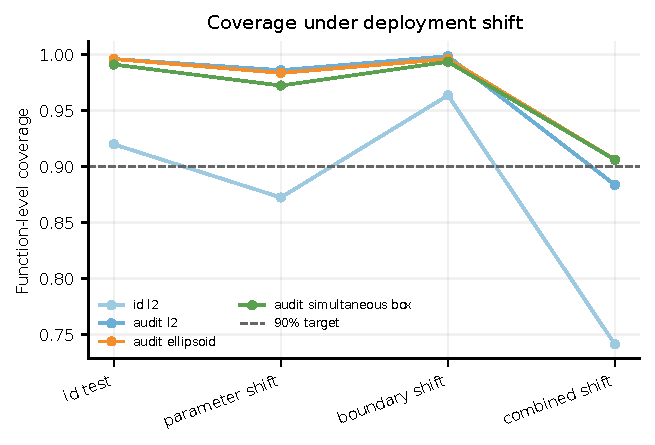
\includegraphics[width=0.72\linewidth]{../../results/fno_burgers_seed27/figures/fno_06_coverage_by_shift.pdf}
\caption{Realized one-step coverage across in-distribution, viscosity-shift,
boundary-shift, and combined-shift test sets. Source calibration degrades most
under combined shift; deployment-audit geometries recover the nominal region
at different widths. Each regime contains 800 test transitions.}
\label{fig:coverage-shift}
\end{figure}

The separately calibrated behavior-trajectory max score attains empirical
coverage 0.88 on 400 held-out length-10 trajectories at target 0.90. We report
the observed proportion rather than rounding it to the target. Its scope is
the fixed behavior-policy distribution in \cref{eq:trajectory-score}.

\subsection{Closed-loop control under latent actuator shift}

\Cref{tab:control-results} answers RQ2. Every robust controller reduces the
empirical $p90$ relative to nominal MPC, but the ordering depends on geometry.
The audit-box adjoint controller lowers mean cost by $1.89\%$ and empirical
$p90$ by $10.84\%$; audit $L^2$ lowers them by $1.92\%$ and $7.79\%$.
The ellipsoid adjoint and nonlinear adversarial variants improve less. Thus
the result supports geometry-dependent decision benefit, not universal
dominance of decision weighting or nonlinear inner maximization.

\begin{table}[t]
\centering
\small
\caption{Closed-loop cost over 24 matched actuator-gain cases. Changes are
relative to nominal MPC; lower is better.}
\label{tab:control-results}
\begin{tabular}{lrrrrr}
\toprule
Controller & Mean & Mean change & $p90$ & $p90$ change & Mean $|a|$\\
\midrule
Nominal MPC & 0.5797 & -- & 1.0752 & -- & 1.278\\
Source-$L^2$ robust & 0.5724 & $-1.27\%$ & 1.0250 & $-4.66\%$ & 1.185\\
Audit-$L^2$ robust & 0.5686 & $-1.92\%$ & 0.9914 & $-7.79\%$ & 1.115\\
Ellipsoid-adjoint & 0.5747 & $-0.88\%$ & 1.0201 & $-5.12\%$ & 1.230\\
Box-adjoint & 0.5688 & $-1.89\%$ & 0.9586 & $-10.84\%$ & 1.101\\
Adversarial ellipsoid & 0.5764 & $-0.58\%$ & 1.0532 & $-2.04\%$ & 1.262\\
\bottomrule
\end{tabular}
\end{table}

\begin{figure}[t]
\centering
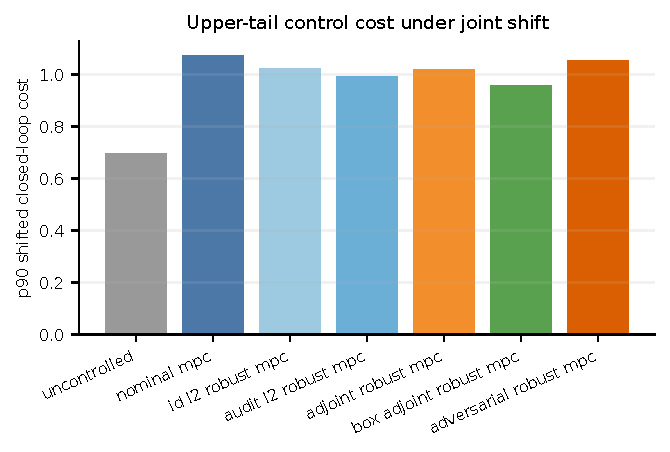
\includegraphics[width=0.69\linewidth]{../../results/fno_burgers_seed27/figures/fno_03_control_p90_cost.pdf}
\caption{Empirical $p90$ closed-loop cost for the matched combined-shift
actuator-gain sweep. The simultaneous-box adjoint controller gives the largest
tail reduction, while the nonlinear adversarial controller is not best in
this finite compute budget.}
\label{fig:control-p90}
\end{figure}

\subsection{High-dimensional Navier--Stokes field audit}

On the official $128\times128$ test set, the base FNO has mean relative
$L^2$ error 0.1635. The max-type multiplier is $q_{0.90}=30.679$;
simultaneous test coverage is 0.883 and mean full coordinate-band width is
4.3409. The pointwise disagreement scale correlates only $r=0.169$ with
absolute error. This is a useful negative result: a valid score construction
can remain inefficient when the maximum spans 16,384 coordinates and the
local scale weakly ranks residual magnitude.

\begin{table}[t]
\centering
\small
\caption{Independent-test Navier--Stokes field-UQ results. No action channel
is available, so no control metric is reported.}
\label{tab:ns-results}
\begin{tabular}{rrrrr}
\toprule
Relative $L^2$ & $q_{0.90}$ & Simultaneous coverage & Full width & Scale--error $r$\\
\midrule
0.1635 & 30.679 & 0.883 & 4.3409 & 0.169\\
\bottomrule
\end{tabular}
\end{table}

\begin{figure}[t]
\centering
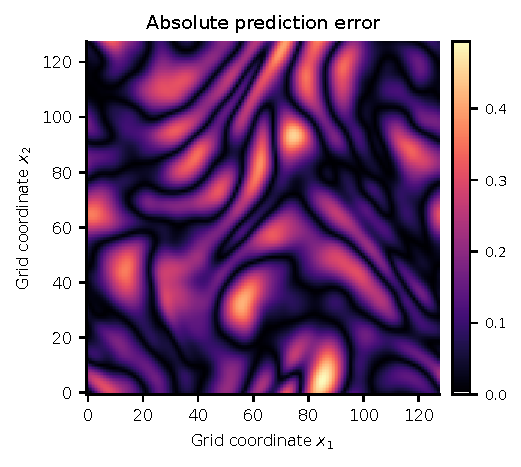
\includegraphics[width=0.56\linewidth]{../../experiments/ns2d_colab_v2/figures/ns2d_04_absolute_error.pdf}
\caption{Representative absolute error of the two-dimensional FNO prediction.
Errors are spatially structured rather than uniform, motivating a local scale;
the following quantitative association test shows that the learned scale only
weakly tracks them.}
\label{fig:ns-error}
\end{figure}

\begin{figure}[t]
\centering
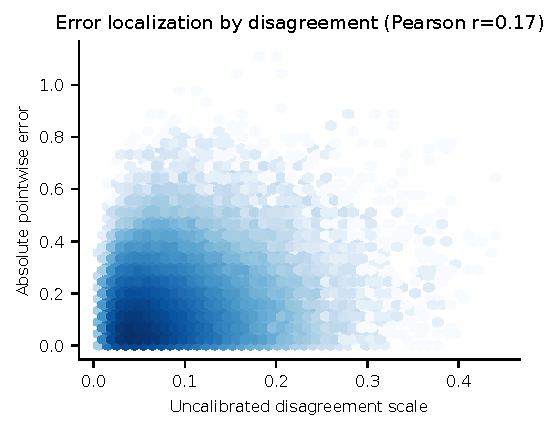
\includegraphics[width=0.63\linewidth]{../../experiments/ns2d_colab_v2/figures/ns2d_11_error_scale.pdf}
\caption{Pointwise perturbation scale versus absolute error on the independent
Navier--Stokes test split. Pearson $r=0.169$ reveals weak localization and
helps explain the large simultaneous conformal multiplier.}
\label{fig:ns-association}
\end{figure}

\subsection{Value-gap scaling and theorem audit}

RQ3 is tested independently of conformal calibration. For the scalar witness
$G(x)=L_Gx$, $\widehat G(x)=L_Gx+\epsilon$, and reward
$-L_r|x|$, the fixed-policy bound is attained. Across six values each of
$\epsilon$ and $\gamma$, the log--log slope is 1.000 in $\epsilon$. After
normalizing the value gap by $\gamma\epsilon$, the slope against effective
horizon $(1-\gamma)^{-1}$ is 2.000, with maximum relative numerical error
$2.55\times10^{-15}$. The experiment verifies the theorem's quantity, not a
conformal consequence.

\begin{figure}[t]
\centering
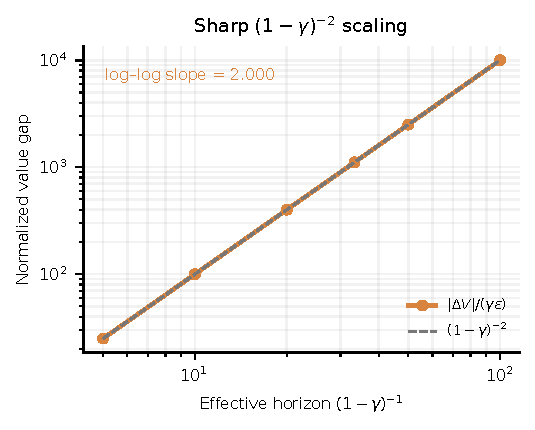
\includegraphics[width=0.55\linewidth]{../../experiments/reward_value_gap_colab_final/figures/value_02_discount_scaling.pdf}
\caption{Sharp deterministic scaling audit. Normalizing by
$\gamma\epsilon$ exposes the predicted quadratic dependence on the effective
discount horizon. The generic policy-transfer bound is twice the fixed-policy
witness plus optimization error.}
\label{fig:value-scaling}
\end{figure}

For ten controlled Burgers rollouts with an exactly injected one-step error,
the maximum observed gap-to-finite-horizon-bound ratio is 0.359. On the learned
FNO's finite visited set, the maximum and mean gap-to-local-envelope ratios are
0.124 and 0.028. These are empirical local audits, not global PDE certificates.

\subsection{Independent value-bound comparison}

RQ5 compares four raw constructions after each is scaled on 60 calibration
trajectories to the same 90\% value-level target, then evaluated on 160
independent trajectories at horizon 20 and $\gamma=0.95$. The local recursion
has the smallest mean bound (0.0870) at 0.944 coverage. Adjoint support is
wider (0.2035) at 0.925 coverage. The fitted curvature coefficient is zero, so
the last two rows coincide. Decision weighting can improve a controller
without producing the tightest scalar value certificate.

\begin{table}[t]
\centering
\small
\caption{Independent-test bound comparison. Utilization is observed value gap
divided by the reported bound. Coverage must be read together with width.}
\label{tab:bounds}
\begin{tabular}{lrrrrr}
\toprule
Method & Coverage & Mean bound & Median $\eta$ & $p90$ $\eta$ & Max $\eta$\\
\midrule
Global maximum & 0.938 & 0.0987 & 0.210 & 0.688 & 3.919\\
Local recursion & 0.944 & 0.0870 & 0.322 & 0.788 & 2.190\\
Adjoint support & 0.925 & 0.2035 & 0.265 & 0.854 & 1.766\\
Adjoint + curvature & 0.925 & 0.2035 & 0.265 & 0.854 & 1.766\\
\bottomrule
\end{tabular}
\end{table}

\begin{figure}[t]
\centering
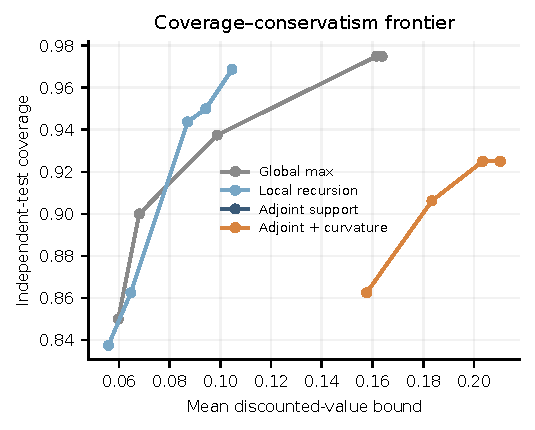
\includegraphics[width=0.59\linewidth]{../../experiments/bound_comparison_colab_final/figures/bound_06_coverage_mean_frontier.pdf}
\caption{Coverage--mean-bound frontier on independent trajectories. A bound is
less conservative only when it is narrower at matched coverage; utilization
alone can be inflated by undercoverage.}
\label{fig:bound-frontier}
\end{figure}

\FloatBarrier
\section{Discussion and limitations}

\paragraph{What the current evidence supports.}
Deployment-audit calibration repairs the source-set failure under compound
shift, but different calibrated geometries lead to different support in the
MPC adjoint direction. In the controlled actuator sweep, this distinction
matters most in the upper tail: the simultaneous box is wide in field space
yet gives the best empirical $p90$ controller. This finding illustrates the
paper's central point: set width in a predictive norm and usefulness in a
decision are not the same ordering.

\paragraph{What the current evidence does not support.}
The Burgers control result is one seed and one matched actuator sweep, not a
multi-seed population claim. The public Navier--Stokes pairs have no action
channel. The ordinary split-conformal theorem requires exchangeability with
the deployment audit and does not cover a later distribution change. Marginal
one-step coverage does not certify the product set queried by MPC, and the
behavior-trajectory result does not cover counterfactual optimized actions.
The deterministic value theorem assumes a uniform error and common
closed-loop Lipschitz constants that were not certified for the learned FNO.
The adjoint robust counterpart is first order unless a uniform curvature
constant is established. Finally, finite CEM and PGD iterations introduce
optimization errors that are measured empirically rather than bounded.

\paragraph{Negative results guide the next experiment.}
The nonlinear adversarial controller is not best; the adjoint scalar bound is
not tighter than the local recursion; the curvature feature adds nothing; and
the Navier--Stokes perturbation scale has weak error association. These outcomes
argue for the following next tests: multiple training/control seeds; audit-size
and shift-severity sweeps; learned low-rank covariance or spectral
function-space sets; policy-coupled trajectory calibration; and a controlled
two-dimensional PDE with an explicit action channel. Deep ensembles,
probabilistic neural operators, and learned quantile operators should be added
as scale baselines under a matched total label and compute budget
\cite{lakshminarayanan2017ensembles}, probabilistic neural operators
\cite{bulte2025probabilistic}, and calibrated quantile operators
\cite{ma2024calibrated}.

\section{Conclusion}

The value of this work is not a new neural-operator block. It is a falsifiable
interface between prediction, uncertainty, and action. A perturbation-derived
scale is first calibrated on a disjoint deployment audit to form a joint
dynamics set over the discretized field. The set is then queried in the
directions that change the finite-horizon objective, either analytically
through exact support functions or numerically through adversarial rollouts.
Finally, predictive coverage, deterministic value propagation, and closed-loop
control are evaluated as separate claims.

The controlled-Burgers results show that this interface can improve empirical
tail cost, but that the benefit is geometry-dependent and does not follow from
coverage alone. The Navier--Stokes stress test shows the opposite pressure:
simultaneous high-dimensional validity can demand wide sets when the local
scale is weak. Together, these results sharpen the research question. The next
advance should not merely produce a narrower prediction band; it should learn
a function-space ambiguity geometry whose calibrated support is both valid for
the deployment regime and useful for the decisions the controller actually
makes.

\begingroup
\footnotesize
\setlength{\bibsep}{2pt}
\bibliographystyle{plain}
\bibliography{references}
\endgroup
\end{document}
